\documentclass[conference,compsoc]{IEEEtran}
\newcommand\tab[1][0.75cm]{\hspace*{#1}}
\usepackage[utf8]{inputenc}
\usepackage[table,xcdraw]{xcolor}

%\ifCLASSOPTIONcompsoc
   \usepackage[nocompress]{cite}
%\else
 
\usepackage{cite}
\usepackage{url}
%\fi


\usepackage[pdftex]{hyperref}


% *** GRAPHICS RELATED PACKAGES ***

\ifCLASSINFOpdf
   \usepackage{graphicx}
   \graphicspath{{files/}}
  
\else
 
\fi
% correct bad hyphenation here
\hyphenation{op-tical net-works semi-conduc-tor}

%********** Começo do documento ************88

\begin{document}



\title{\resizebox{!}{0.75cm}{Relatório Final}\\Reconhecimento facial em tempo real aplicado no Restaurante Universitário da Faculdade Gama.}



\author{
\IEEEauthorblockN{João Vitor Rodrigues Baptista}
\IEEEauthorblockA{15/0013329\\UnB - FGA \\
Brasília, Brasil \\
Email: jvrbaptista@live.com }
\and
\IEEEauthorblockN{Igor Sousa Nunes de Oliveira}
\IEEEauthorblockA{15/0011971\\
UnB - FGA \\
Brasília, Brasil\\
Email: igorsno97@gmail.com }}
\maketitle

% As a general rule, do not put math, special symbols or citations
% in the abstract

\begin{abstract}
Aplicação de monitoramento facial em tempo real no Restaurante Universitário da Faculdade Gama utilizando Raspberry pi para melhorar a eficiência do sistema e evitando problemas no acesso de usuários. \cite{referencia:3} 
\end{abstract}
\IEEEpeerreviewmaketitle
\section{Introdução}
Sistemas de controles de acesso são uma ferramenta muito importante na contemporaneidade para a segurança de ambientes controlados, produtos, pessoas ou para de maneira simples um controle de tempo dos usuários do sistema. \cite{referencia:7}

Com o passar do tempo notou-se que uma boa forma de identificação seria através de padrões do ser humano de maneira que a chave de acesso sempre estaria com usuário. Um dos padrões bastante associados com a identificação foi a digital, e desde cedo estudada para se entender padrões já que a  mesma é diferente para cada pessoa, sensores biométricos se tornaram bastante utilizados desde celulares até mesmo cofres. Um padrão que está sobre um grande estudo na contemporaneidade são padrões reconhecidos por imagem como a face e em certas aplicações até mesmo a leitura de padrões na iris do usuários.\cite{referencia:7}

A tecnologia entrou em um padrão de evolução buscando maior conforto, acessibilidade, velocidade e segurança
para seus usuários, o reconhecimento facial se tornou uma poderosa ferramenta na aquisição de dados por 
não precisar de módulos sensores de uso específicos como o leitor biométrico. 

Em países como a China onde o investimento na área de segurança e processamento digital de imagens conseguiram criar uma rede de câmeras que identificam pessoas a distancia, então o processo de transformar o usuário na própria chave do sistema
foi a melhor saída para uma maior segurança do sistema, praticidade e até mesmo melhoras no fluxo de filas em 
ambientes controlados entre outros.\cite{referencia:4} \cite{referencia:5} 

\section{Justificativa}
Na  contemporaneidade o grande fluxo de pessoas em diversos ambientes controlados levantou questões sobre a eficiência dos métodos utilizados, em geral existe um custo associado individualmente para cada usuário possua uma chave(no caso de cartões, tarjas magnéticas, transponders entres outros).  A segurança é uma outra característica fundamental ao ambiente de maneira que os métodos comumente utilizados possuem uma maior probabilidade de serem fraudados.

Motivado pela modernização implementada no controle de acessos a escolha de uma parâmetro de identificação biométrico se torna de grande utilidade como chave do sistema, pois o usuário se torna chave do sistema o que tira do projeto um custo adicional pertencente a cada passe que deve utilizado individualmente para um controle mais efetivo do ambiente.

Com uma pesquisa sobre o custo beneficio de cada tipo de leitura biométrica a escolhida como tema deste projeto pelo baixo custo e boa eficiência de maneira que uma das suas principais vantagens é a facilidade de identificação de fraude por terceiros que estejam no mesmo lugar. Diante do exposto a utilização do reconhecimento facial torna mais cômodo para os usuários e para o proprietário do sistema, devido uma maior eficiência e automatização do mesmo em comparação a outros métodos.
 
 \section{Objetivos}
Tornar o controle de acesso ao Restaurante Universitário da Faculdade Gama eficientes tornando o fluxo de pessoas que entram mais rápido e automatizando o controle de usuários.
Identificar as pessoas que entram e saem além de poder ter
controle dos tempos de acessos de cada pessoa individualmente e armazenar em um banco de dados.
Monitorar pessoas que tentem entrar no ambiente de forma
indevida e impedir a entrada de usuários quem não tenham a
devida autorização.

\begin{figure}[!ht]
		\centering
		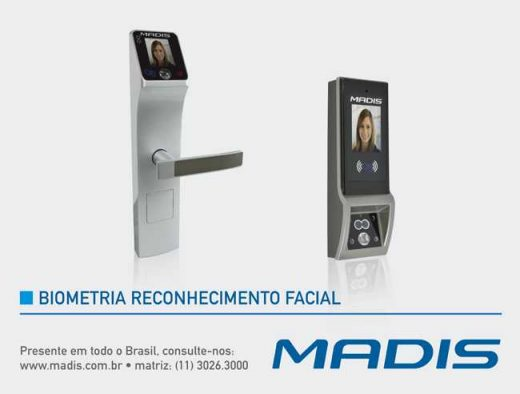
\includegraphics[scale=0.25]{exemplo.jpg}
		\caption{Produto semelhante já encontrado no mercado \cite{referencia:8}}
		%\label{Rotulo}
\end{figure}

 
 
 \section{Hardware}
 
Em termos de melhoria e mudanças de hardware substituiu-se a webcam usadas para teste e foi implementado a câmera especifica da raspberry. Ao fazer essa modificação pode-se notar uma melhora no desempenho tanto da velocidade quanto de qualidade do cadastramento e no reconhecimento. Portanto, houve uma melhora geral do protótipo.   
 
 \begin{figure}[!ht]
		\centering
		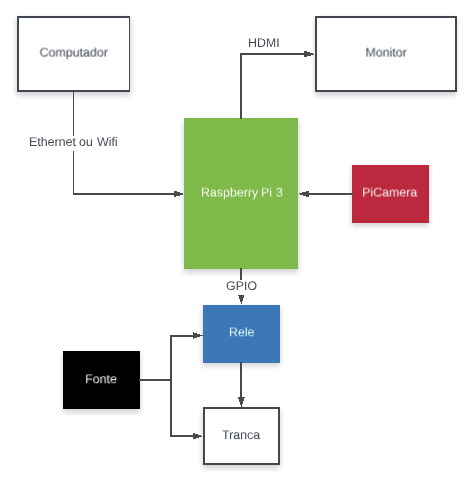
\includegraphics[scale=0.25]{diagrama_de_hardware.png}
		\caption{Diagrama de Hardware}
		%\label{Rotulo}
\end{figure}

Como esta indicado no diagrama de hardware do projeto na figura 2. Ligou-se a raspberry pi 3 como entrada HDMI para mostrar a interface gráfica para o usuário já que será indicado se o usuário foi reconhecido. A PiCamera foi ligada como entrada do sistema, pois a partir dos dados de entrada providos o sistema faz o julgamento se o usuário esta ou não cadastrado no banco.
	
	Uma vez que o usuário foi reconhecido e tem créditos o suficiente o sistema manda um sinal para abrir um rele 5V que esta sendo a chave de uma tranca solenoide de 12v. O painel de modificações do banco de dados é acessado através de um computador ligado via ethernet ou Wifi com a raspberry.
	




 \section{Software}

O software tem como o principio básico três partes que consiste em cadastrar: recebe o nome, matricula e fotos do aluno, treinar as imagens e reconhecer a imagens que entram através da PiCamera com as imagens do banco de dados. Baseado nessas partes básicas foram adicionados outras funcionalidades para manipular o banco de dados.

\begin{figure}[!ht]
		\centering
		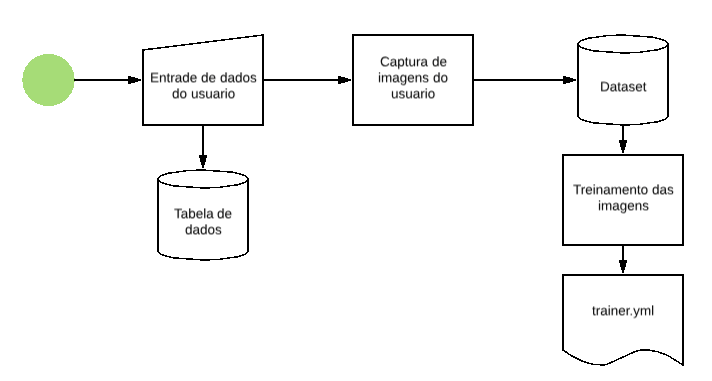
\includegraphics[scale=0.25]{Cadastro.png}
		\caption{Fluxograma do funcionamento do cadastro.}
		%\label{Rotulo}
\end{figure}

Na figura 3 é apresentado o fluxo de cadastro, onde o aluno digita o nome e a matricula, em seguida são tiradas 30 fotos que são salvas para um dataset com a posição do vetor sendo o nome da imagem, em seguida são feitas os processamentos de imagens da biblioteca opencv.

\begin{figure}[!ht]
		\centering
		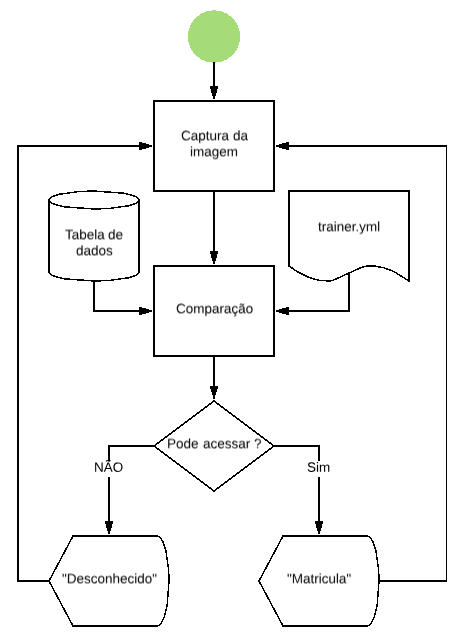
\includegraphics[scale=0.25]{Reconehcimento.png}
		\caption{Fluxograma do funcionamento do reconhecimento da biblioteca opencv.}
		%\label{Rotulo}
\end{figure}

Na figura 4 é mostrado o fluxo de reconhecimento de imagem. A partir do arquivo gerado pelo treinamento do dataset, a biblioteca opencv faz o reconhecimento entre o que esta sendo gravado e as imagens que foram treinadas com uma precisão ajustável, que depende tanto da qualidade da câmera, como das condições do ambiente e da lógica de validação. 

\begin{figure}[!ht]
		\centering
		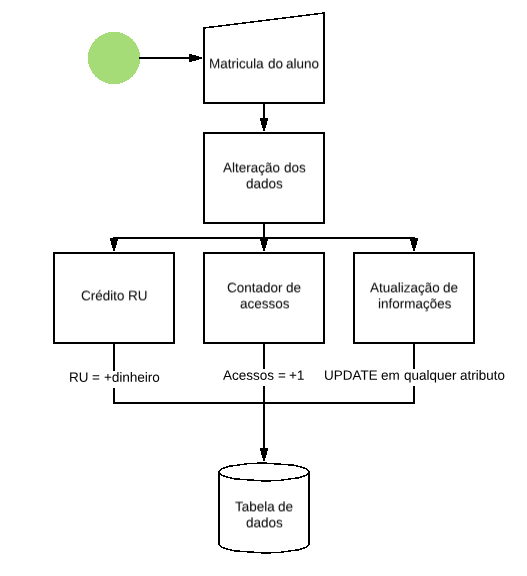
\includegraphics[scale=0.25]{Banco_de_dados.png}
		\caption{Fluxograma do funcionamento banco de dados.}
		%\label{Rotulo}
\end{figure}

A figura 5 mostra algumas funções de manipulação do banco de dados que são acessadas pelo computador através de uma aplicação web ligado com a raspberry mostrado na figura 6. As funções implementadas são: Adicionar crédito, apagar um cadastro e vizualização dos logs. 

\begin{figure}[!ht]
		\centering
		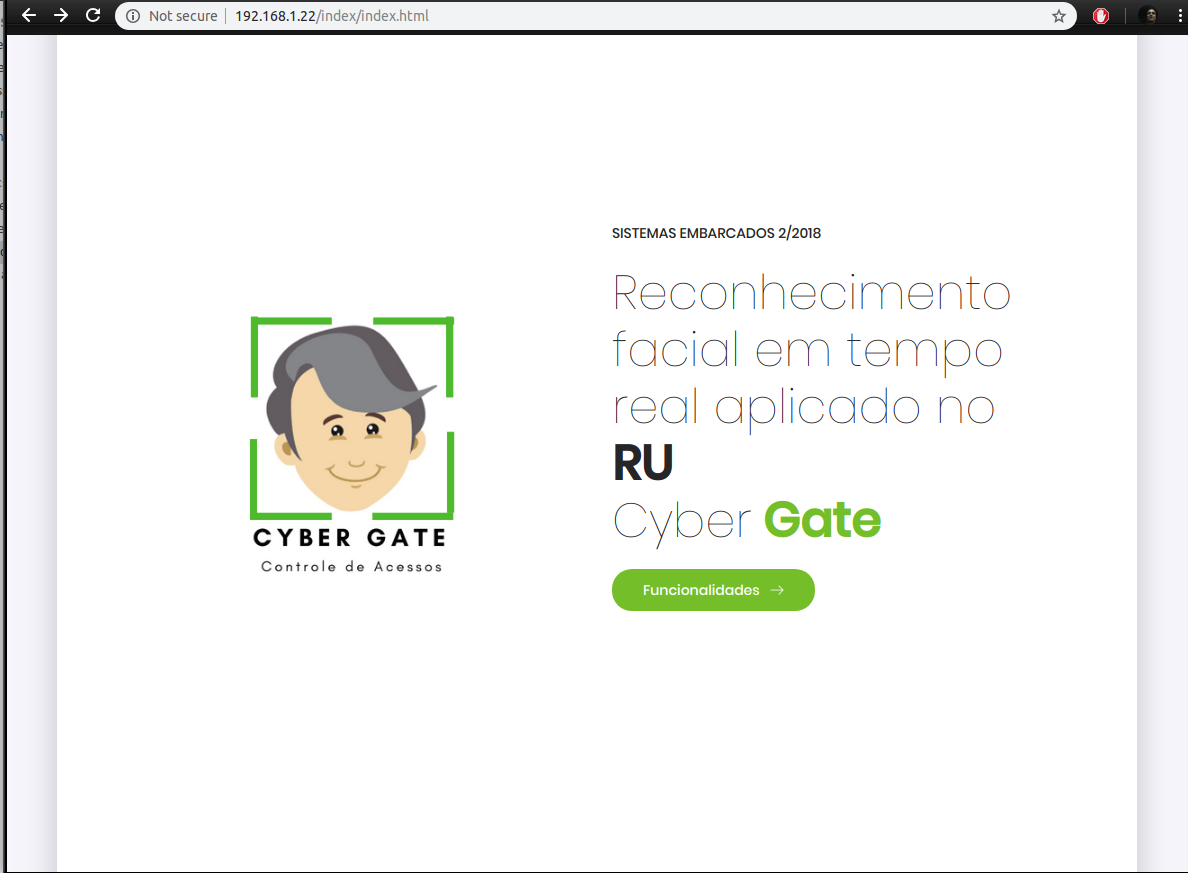
\includegraphics[scale=0.15]{web_app.png}
		\caption{Web aplicação para manipular o banco de dados.}
		%\label{Rotulo}
\end{figure}

O banco de dados esta organizado de acordo com a tabela de CADASTROS que possui cinco atributos, ID, NOME, MATRICULA, RU e ACESSOS como mostrado na figura 7. Podendo, se necessário, ser adicionado novos atributos.  


 \begin{figure}[!ht]
		\centering
		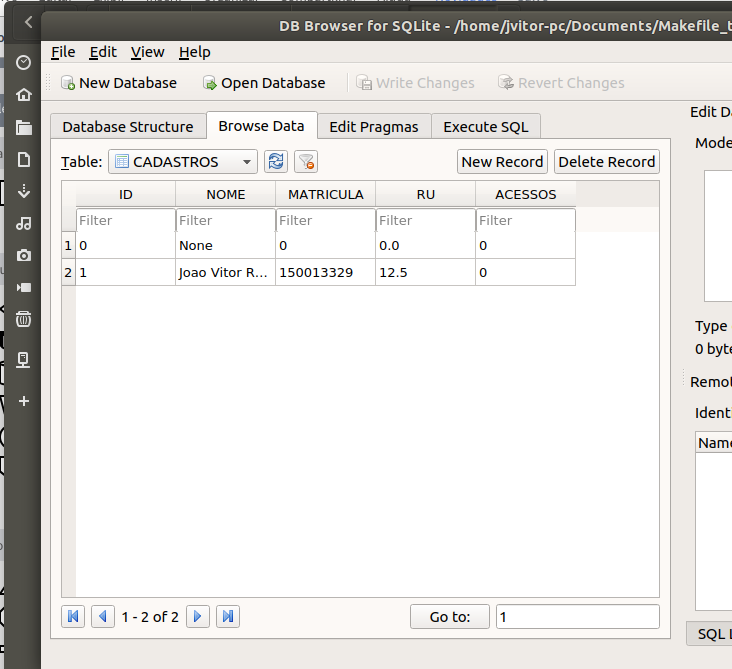
\includegraphics[scale=0.25]{infra_database.png}
		\caption{Atributos do banco de dados.}
		%\label{Rotulo}
\end{figure}

A interface foi desenvolvida com o objetivo de ter uma interação com o usuário e não deixar apenas a imagem da câmera. Como esta indicado nas figuras 8, 9 e 10 é mostrado a  interface é em conjunto com a câmera de captação, a interface indica o nome, matricula, créditos restantes e se ele pode ou não acessar o ambiente. Quando o usuário esta no processo de validação a interface apresenta que esta "identificando" o usuário.  


Todos os codigos e figuras estão no repositório no GitHub, através do link:
\href{https://github.com/helpthx/Sistemas_Embarcados/tree/master/2_PCs/Ponto_de_Controle_3/Arquivos}{helpthx}

\section{Requisitos}
\begin{itemize}
   \item Um microcontrolador no qual a escolha de projeto é o Raspberry pi 3 B. 
   \item Um módulo de câmera para a Raspberry.
   \item Um display para se mostrar as informações necessárias.
   \item Uma estrutura para proteger o sistema.
   \item Cabo HDMI.
   \item Modulo rele 5V.
   \item Fonte de alimentação.
   \item Tranca solenoide 12V
   \item Conexão com a internet.
   \item Software de reconhecimento facial.
   \item Software  para criação de logs e registros.
   \item  Infraestrutura do servidor para criação e alteração do banco de dados.
   \item Banco de dados para guardar informações do usuário(Fotos, créditos e acessos).
   \item Testador de continuidade.
 \end{itemize}
 
\section{Benefícios}
Processo com maior segurança para os usuários, onde não é necessário  memorizar senhas ou carregar algum tipo de chave, o traço pessoal é mais difícil de ser clonado ou copiado o que trás maior segurança para todos os usuários do sistema.

Custo semelhante ou inferior ao de sistemas de controles de acessos, valorização da modernização, melhoria do design e apresentação do ambiente.

\section{Resultados}

Foi implementado um sistema de validação de \emph{frames} consecutivos que funciona de forma que se 5 \emph{frames} consecutivos obtiverem uma taxa de confiabilidade de mais de 70\% o código avança para os próximos passos de liberar ou não o usuário. Porem o essa parte ainda esta na fase de testes e calibração para implementar o melhor sistema de validação de entrada. Na figura 9 pode-se observar o sistema de validação tentando identificar os 5 \emph{frames} consecutivos mostrando a mensagem "Identificando". 


\begin{figure}[!ht]
		\centering
		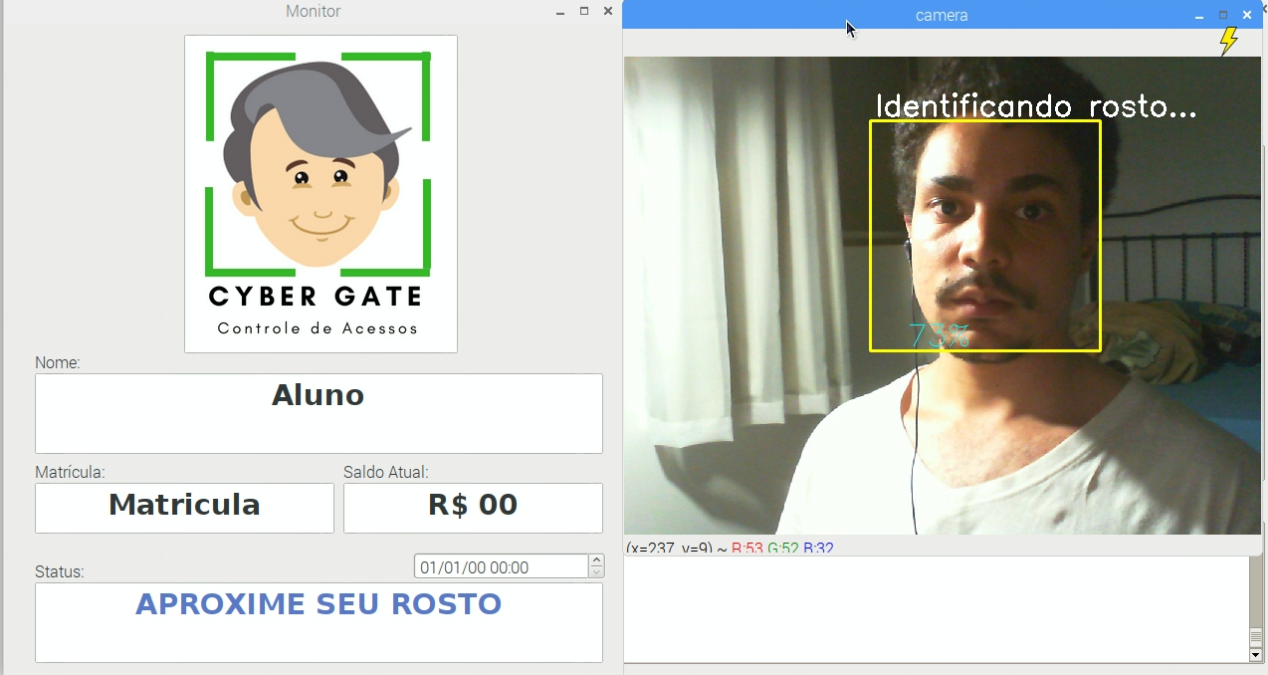
\includegraphics[scale=0.15]{identificando.png}
		\caption{Processo de validação com frames consecutivos}
		%\label{Rotulo}
\end{figure}

	Após testes com a nova câmera notou-se que a melhoria na confiabilidade do sistema foi menor do que o esperado, mesmo com uma melhora na resolução outros fatores ainda interferem o sistema de maneira mais extensa do que o esperado. A iluminação e interferências de imagens em um possível segundo plano de imagem atrás da pessoa a ser identificada foi de fato maior analisada nos teste apresentados nesses ponto de controle, a iluminação muito baixa torna mais difícil a detecção dos detalhes do rosto o outro extremo também atrapalha o total funcionamento do sistema, este problema é comum na maioria dos sistemas de reconhecimento facial e vêm sendo estudado para melhor criação de algoritmos que não seja atrapalhados pela luz. 
	
	\begin{figure}[!ht]
		\centering
		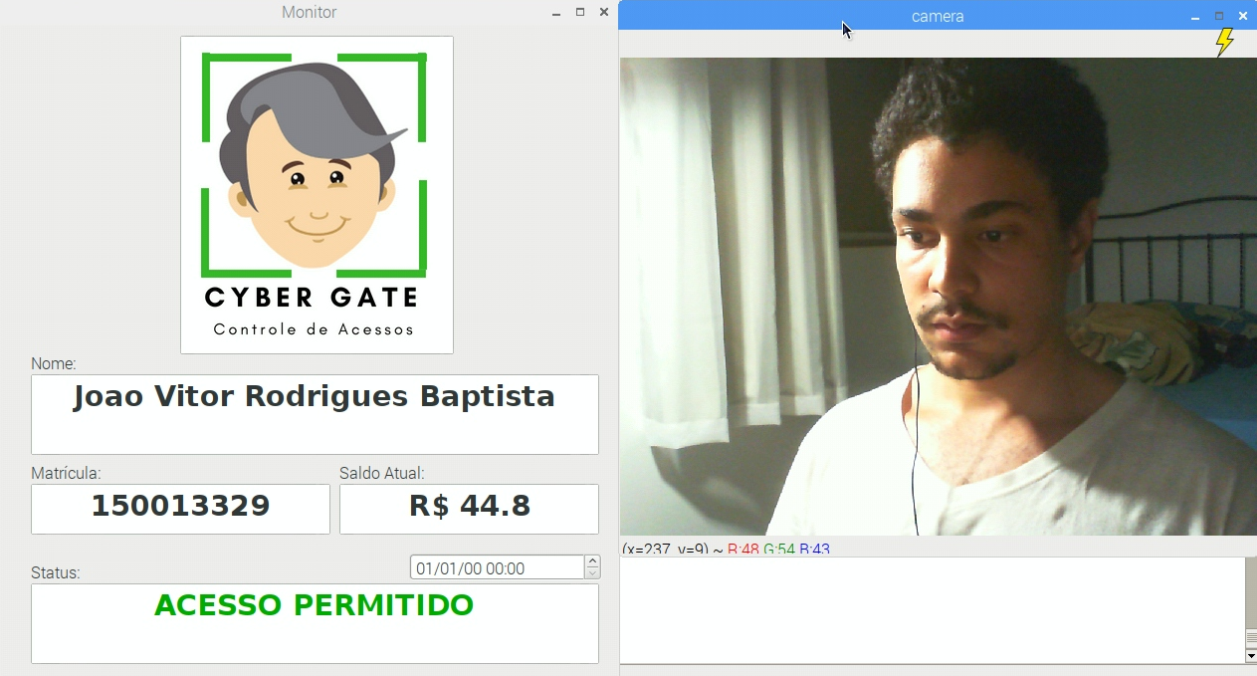
\includegraphics[scale=0.20]{interface.png}
		\caption{Interface que irá interagir com o usuario}
		%\label{Rotulo}
\end{figure}
	
	O plano de imagem atrás do usuário realmente foi outro problema a ser notado, pois o sistema busca imagens que consiga comparar com um rosto, então a movimentação de objetos e pessoas atrás da pessoa a ser identificada atrapalha o processo tornando a necessidade de um maior tempo para o reconhecimento e em casos extremos não deixando o sistema reconhecer um dos rostos.
	
	\begin{figure}[!ht]
		\centering
		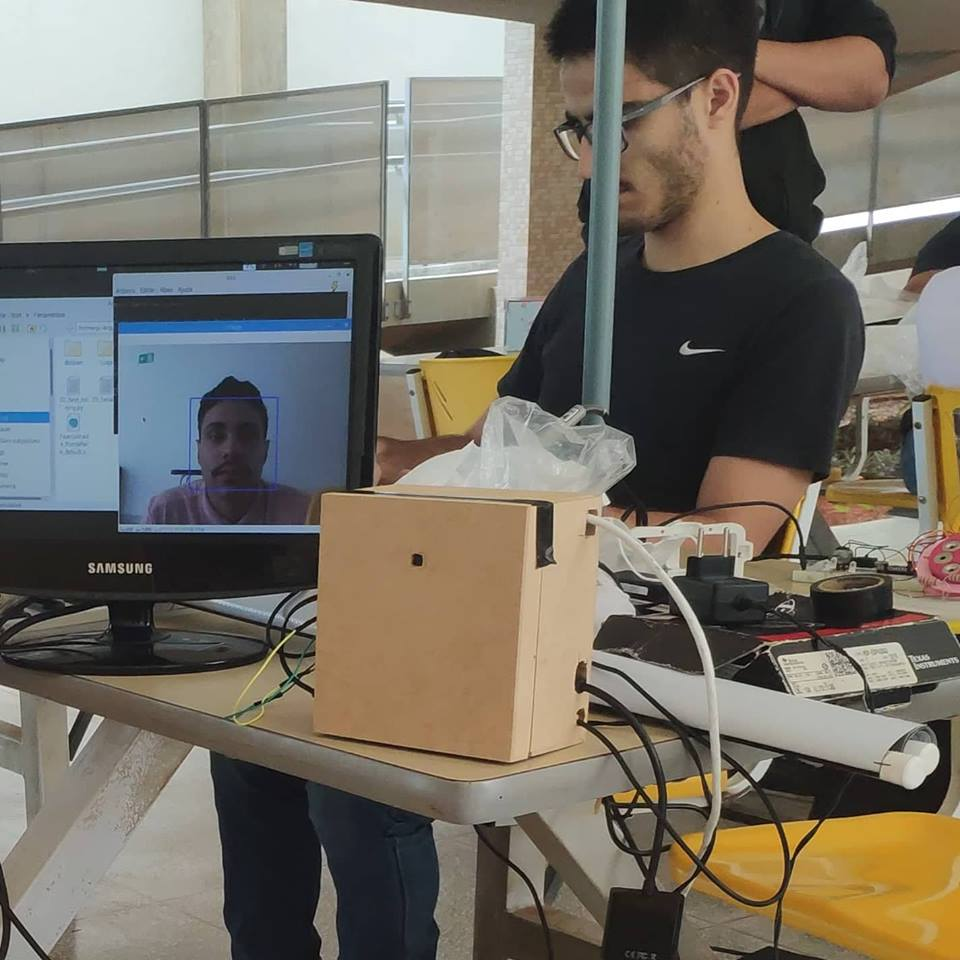
\includegraphics[scale=0.20]{projeto.jpg}
		\caption{Estrutura do prototipo}
		%\label{Rotulo}
\end{figure}



Para a entrega final do protótipo foi feita uma estrutura de madeira , mostrada na figura 10, que comporta a câmera pi, raspberry e tem entradas para todos os cabos que são utilizados. Assim como todos os ajustes de validação da imagem que leva em conta a qualidade da câmera e o numero de frames utilizados.

\begin{figure}[!ht]
		\centering
		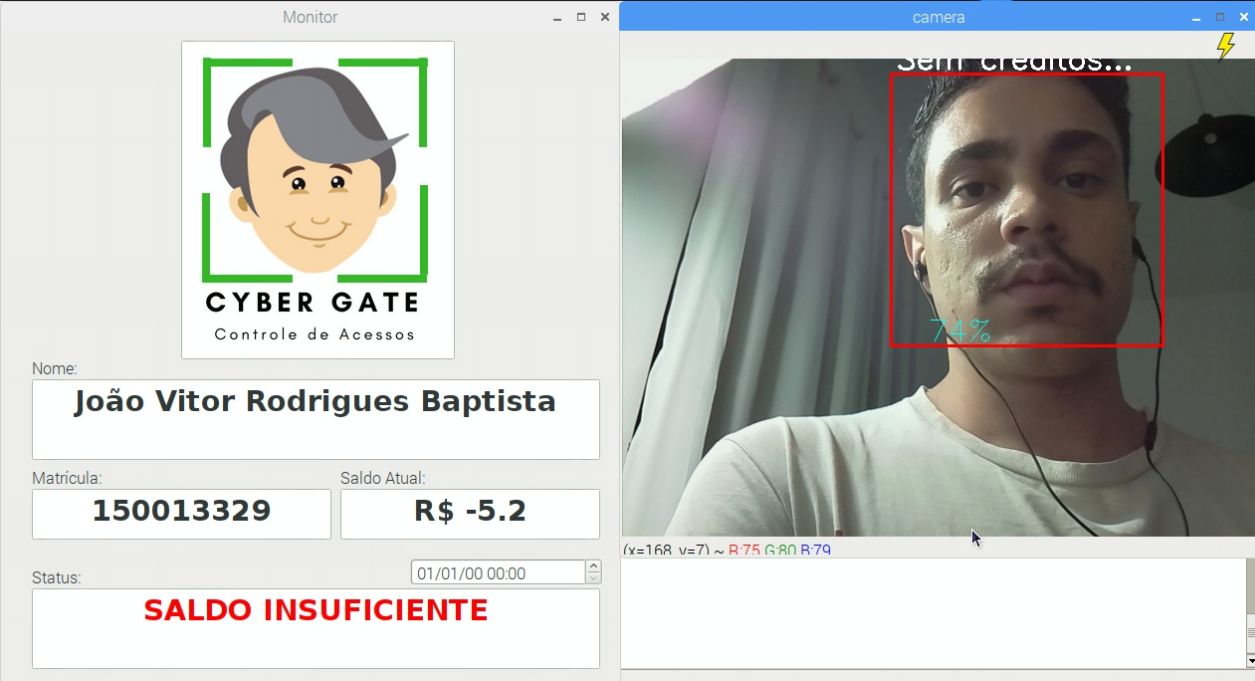
\includegraphics[scale=0.20]{camera_invalido.png}
		\caption{Mensagem quando o usuário não tem créditos suficiente.}
		%\label{Rotulo}
\end{figure}


\section{Conclusão}

A segurança é algo indispensável para a vida na era extremamente digital que vivemos, de maneira que a implementação de sistemas que aumentam a segurança de um ambiente ou procedimento sao sempre bem vindas, principalmente se forem de baixo custo, eficientes e intuitivos ao usuário.

 O protótipo final esta totalmente funcional. O sistema de validação dos frames consiste em verificar 10 amostras não consecutivas, o que possibilitou uma otima segurança em relação a qualidade da camera e o poder de processamento do microcontrolador. Todo o sistema de manipulação via web esta totalmente funcional. 
 
 Em um contexto geral, o protótipo funciona conforme o planejado, porem houve erros de alimentação na tranca da porta, esse problema resultou em reiniciamentos da raspberry. Portanto, não foi possível abrir a porta usando o reconhecimento, porem foi possível ver que o rele estava sendo acionado para abrir a trava. 
 
 Assim, ao desenvolver o prototipo foi notado que esse sistema pode ter varias outras aplicações no mercado de acessos, basta melhorar o desempenho do microcontrolador.  
	  
	  
         

	
%---------------------  ----------------------

%\section{Materiais Utilizados}
%TABELAS AQUI

%\begin{table}[tbp]
%\caption{Tabela 1 - Exemplo}
%\label{my-label}
%\begin{tabular}{ccccc}
%\textbf{Nome}   & \textbf{Nome1} & \textbf{Nome2} & \textbf{Nome3} & \textbf{Nome4} \\
%\textbf{Nome11} & 1              & 2              & 3              & 4              \\
%\textbf{Nome21} & 5              & 6              & 7              & 8              \\
%\textbf{Nome31} & 9              & 10             & 11             & 12            
%\end{tabular}
%\end{table}
%---------------------  ----------------------

%\section{Hardware e Software}

%---------------------  ----------------------
%\subsection{Descrição do Hardware}

%Como é observado no diagrama de blocos, é necessária uma fonte externa para acionar a trava solenoide, pois os 3 volts fornecidos pela placa não é suficiente para fazer o acionamento da trava.

%\begin{figure}[!ht]
%		\centering
%		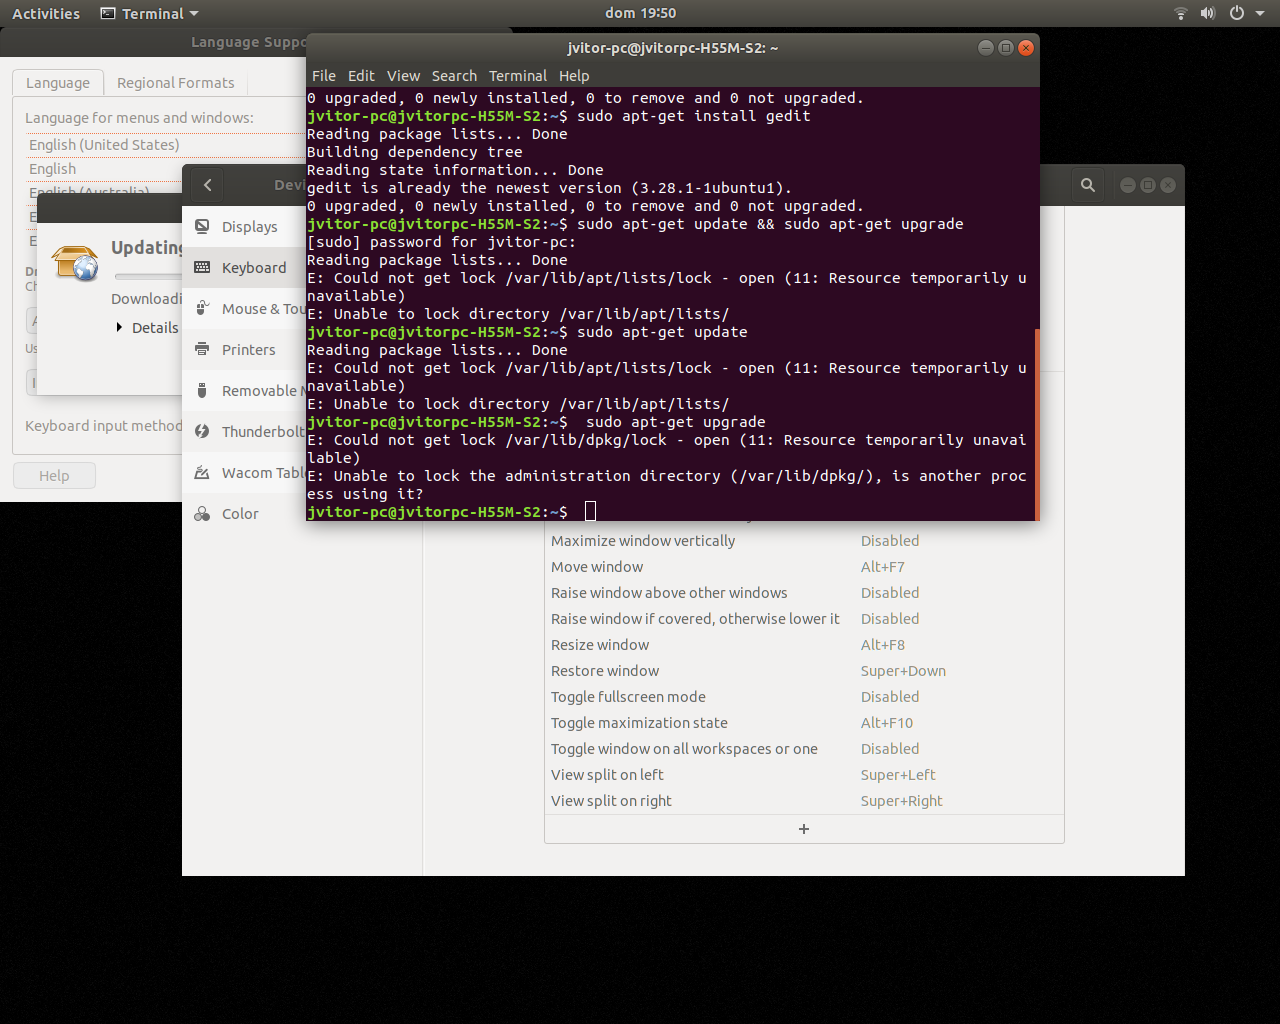
\includegraphics[scale=0.15]{nome_da_figura.png}
%		\caption{Figura 1.}
		%\label{Rotulo}
%\end{figure}

%O resultado foi o esperado, ao passar o tag no leitor RFID, gerou-se um sinal para o relê abrir a tranca eletrônica, através da alimentação de uma bateria de 9 – 12V. 
%Display de Cristal Liquido: Pode ser facilmente implementado no MSP430 utilizando a biblioteca "LiquidCrystal.h". O display será utilizado para exibir as mensagens:

%---------------------  ----------------------


%\subsection{Descrição do Software}
%Para melhor ilustrar o caminho logico deste sistema, foi construído um Diagrama Logico na imagem 5. Para mostrar de maneiras simples a ideia lógica do sistema proposto.
% \begin{figure}[!ht]
%		\centering
%		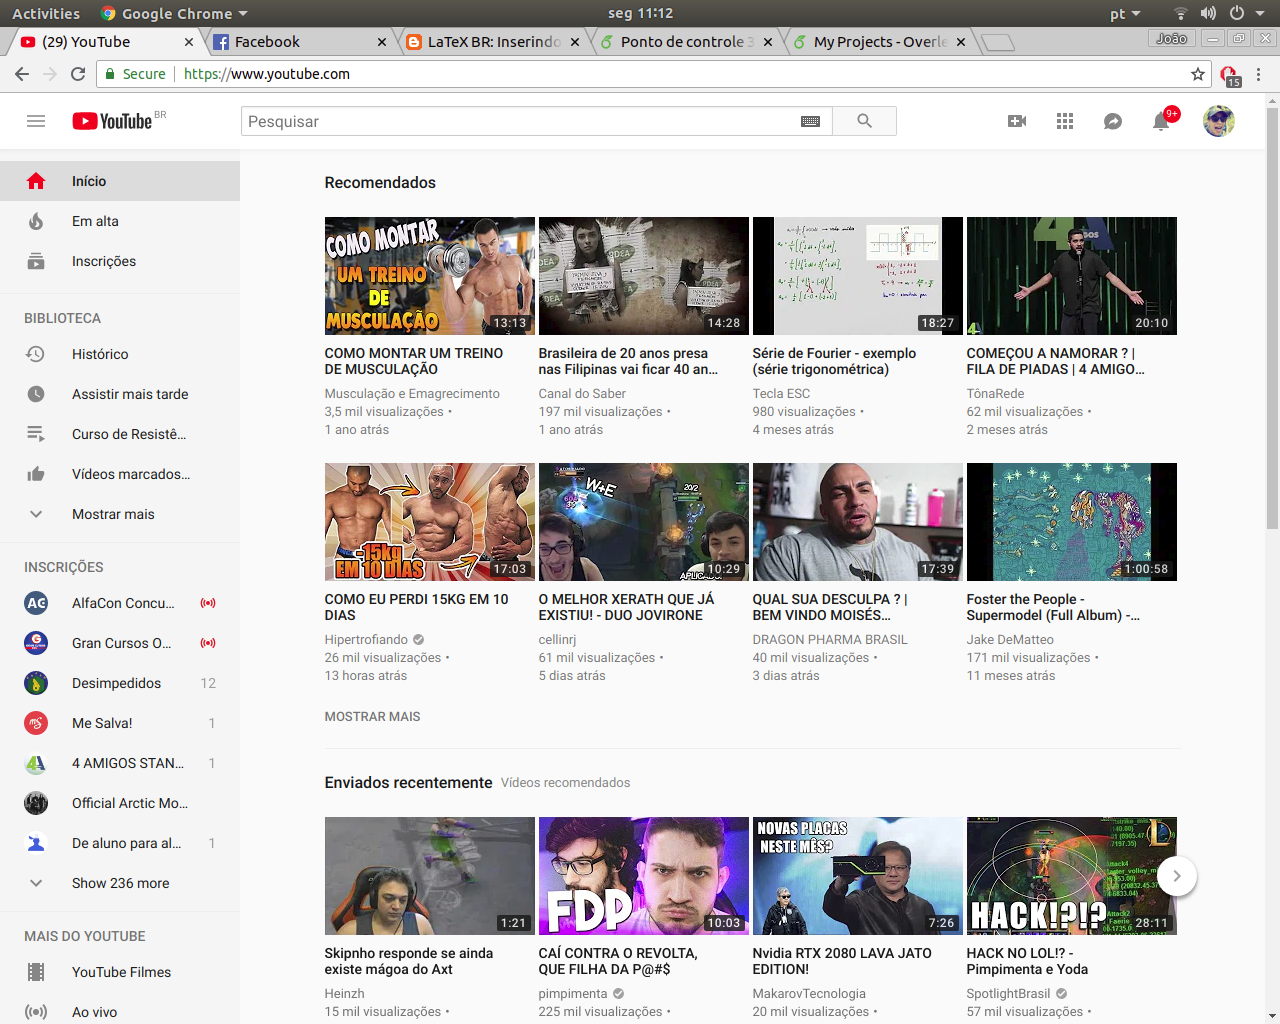
\includegraphics[scale=0.15]{nome_da_figura1.png}
%		\caption{Figura 1}
		%\label{Rotulo}
%\end{figure}

%O Sistema consiste nos seguintes passos:

%\tab 1. Iniciar a comunicação UART com o RC522. Exibindo “RFID LOADING...” ao iniciar.

%\tab 2. Quando o sistema estiver pronto e iniciado exibir “PASSE O CARTÃO”.

%\tab 3. Ler o conteúdo do cartão ou tag.

%\tab 4. Julgar se o cartão ou tag, pode ou não destravar o sistema.

%\tab 5. Destrava o sistema e envia um sinal para o rele, exibe  “BEM VINDO USUARIO”, espera 7 segundos e vai para o loop de leitura.

%\tab 6. Trava o sistema quando o cartão não tem acesso, exibe “ACESSO NEGADO”, volta para o loop de leitura. 



%\begin{figure}[!ht]
%		\centering
%		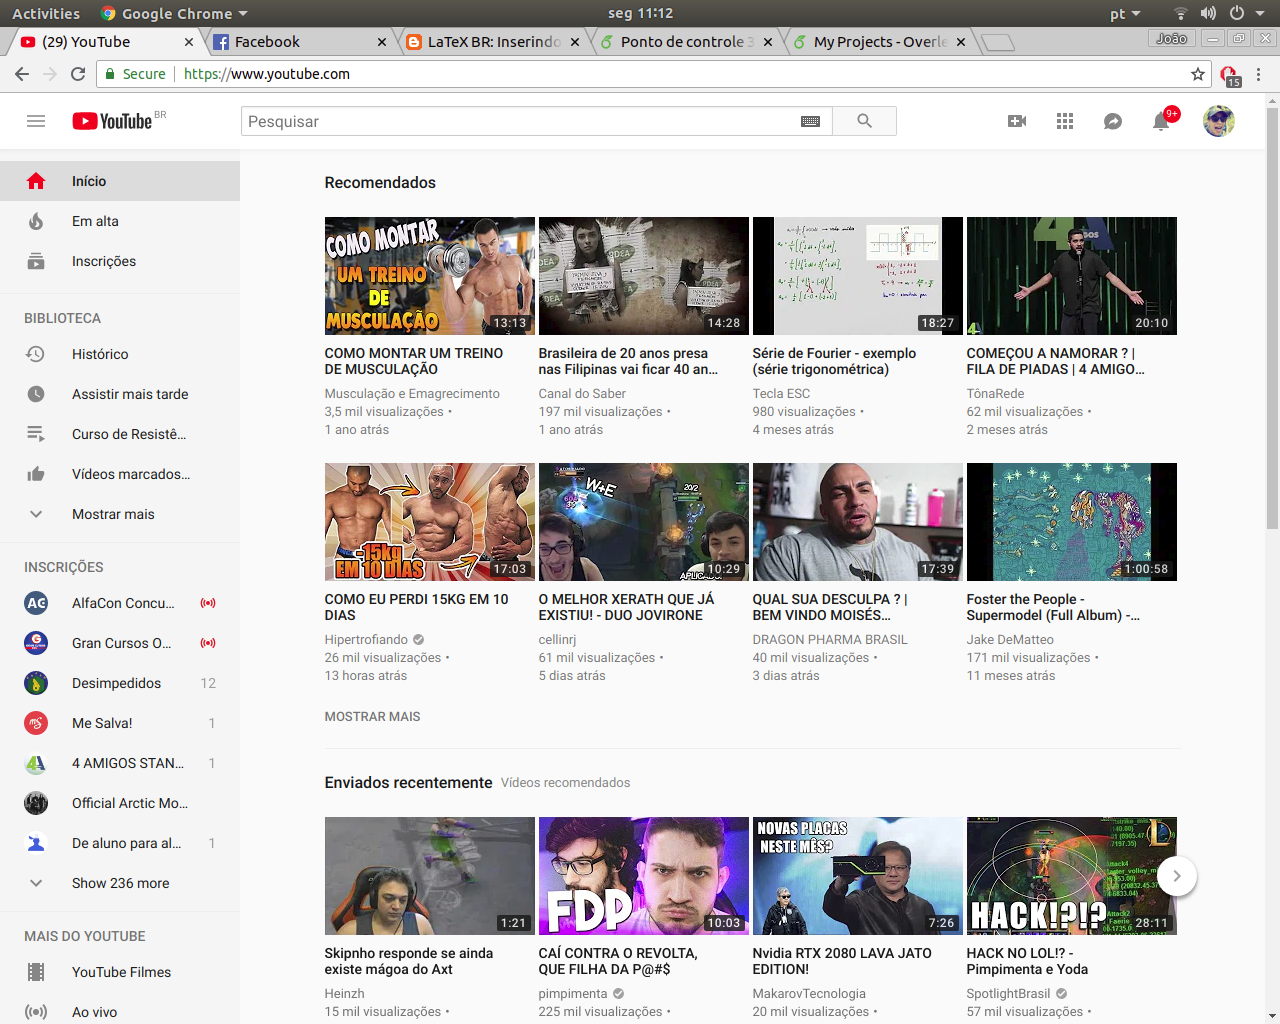
\includegraphics[scale=0.15]{nome_da_figura1.png}
%		\caption{Figura 1}
		%\label{Rotulo}
%\end{figure}

%Os códigos e as figuras estão no GitHub, através do link:\href{https://github.com/helpthx}{https://github.com/helpthx}

%---------------------  ----------------------

%\section{Resultado}
%Os resultados foram conforme o esperado ao se juntar todos os componentes, entretanto houve algum problema na comunicação com o display 16x2, o qual não exibe as mensagens de trava e destrava do sistema de maneira correta, ou seja, em certos momentos caracteres estranhos são mostrados no display. Porem a comunicação entre o RC522, MSP430 e o rele esta totalmente funcional e a trava esta se comportando como deveria. Para os próximos passos será corrigido o problema do display e possivelmente adicionado mais funções ao sistema.

%\begin{figure}[!ht]
%		\centering
%		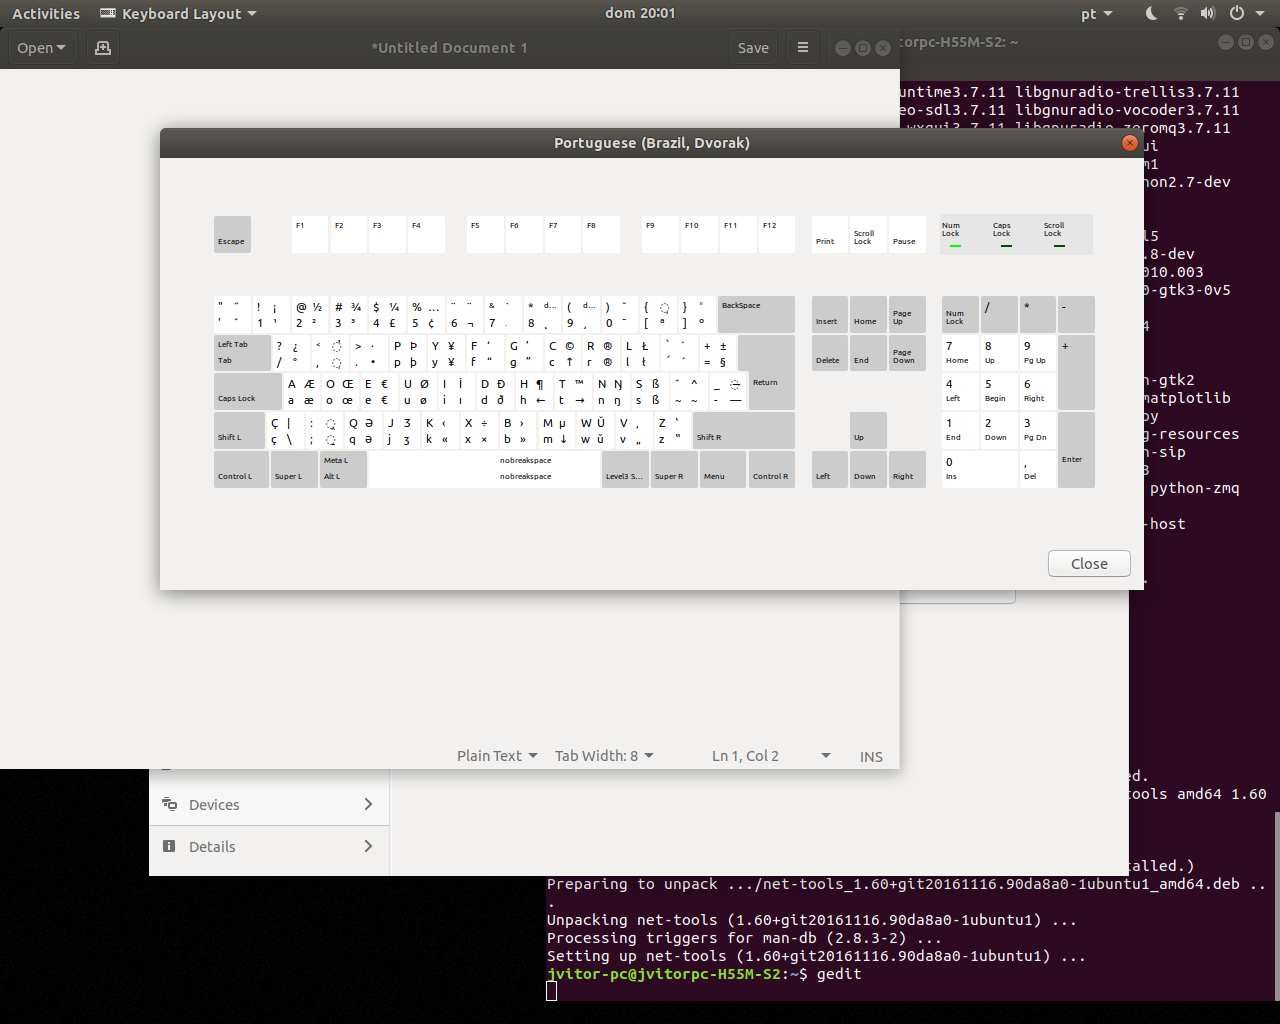
\includegraphics[scale=0.15]{nome_da_figura3.png}
%		\caption{Figura 3}
		%\label{Rotulo}
%\end{figure}

%---------------------  ----------------------

%\section{Relação de Custo}
%Até o presente momento se foi gasto em torno de R\$214,10 para o projeto, o que pode ser extremamente reduzido se as peças fossem compradas com certa antecipação, o MSP comprado direto pelo fornecedor a Texas, dessa maneira fazer com que o preço do projeto reduzido em mais de 50\% do valor atual, os outros componentes se comprando em grandes quantidades consegue-se uma grande redução de preços, o que viabilizaria a construção em maior escala do projeto com um menor preço e com certas melhorias uma possível entrada na concorrência de vendas de produtos pensados para segurança e controle de ambientes, como sendo uma alternativa de baixo custo que poderia ser modificada com necessidades do próprio cliente. \cite{referencia:1}



%-------------------- REFERÊNCIA -----------------

\begin{thebibliography}{1}


%\bibitem{IEEEhowto:kopka}
%H.~Kopka and P.~W. Daly, \emph{A Guide to \LaTeX}, 3rd~ed.\hskip 1em plus
 % 0.5em minus 0.4em\relax Harlow, England: Addison-
%FALTA ARRUMAR AS REFERÊNCIAS


\bibitem{referencia:2}
{TIWARI, Shantnu
\emph{Face Detection in Python Using a Webcam.},
 {Disponivel em:\url{<https://realpython.com/face-detection-in-python-using-a-webcam/>}},{Acesso em: 01 set. 2018.}
}

\bibitem{referencia:3}
{MJROBOT, MJRoBot.
\emph{Real-Time Face Recognition: An End-to-End Project.},
 {Disponivel em:\url{<https://www.hackster.io/mjrobot/real-time-face-recognition-an-end-to-end-project-a10826>.}},{Acesso em: 01 set. 2018.}
}

\bibitem{referencia:4}
{VICENTIN, TISSIANE.
\emph{Projeto usa Raspberry e reconhecimento facial para medir produtividade.},
 {Disponivel em:\url{<https://www.tecmundo.com.br/software/126916-projeto-usa-raspberry-reconhecimento-facial-medir-produtividade.htm>}},{Acesso em: 01 set. 2018.}
}

\bibitem{referencia:5}
{CASSITA, DANIELLE.
\emph{Reconhecimento facial ajuda polícia a identificar suspeito em festival. 2018.},
 {Disponivel em:\url{<https://www.tecmundo.com.br/software/133803-reconhecimento-facial-ajuda-policia-identificar-suspeito-festival.htm>.}},{Acesso em: 01 set. 2018.}
}

\bibitem{referencia:6}
{CHOWDHURY, Nasimuzzaman.
\emph{Access Control of Door and Home Security by Raspberry Pi Through Internet. 2018.},
 {Disponivel em:\url{<https://www.ijser.org/researchpaper/access-control-of-door-and-home-security-by-raspberry-pi-through-internet.pdf>.}},{Acesso em: 01 set. 2018.}
}

\bibitem{referencia:7}
{AXIS, Communications.
\emph{Reconhecimento facial. },
 {Disponivel em:\url{<https://www.axis.com/pt-br/solutions-by-application/facial-recognition>}},{Acesso em: 01 set. 2018.}
}
\bibitem{referencia:8}
{INOVADOR DESDE 1923, MADIS.
\emph{Biometria Reconhecimento Facial.},
 {Disponivel em:\url{<https://www.madis.com.br/produtos/biometria-reconhecimento-facial/>.}},{Acesso em: 19 out. 2018.}
}


\end{thebibliography}




% that's all folks
\end{document}
